\documentclass{standalone}
\usepackage{amsfonts,amsmath,amssymb}
\usepackage[slovene]{babel}
\usepackage[utf8]{inputenc}
\usepackage[T1]{fontenc}
  
\usepackage{tikz, verbatim}
\usepackage{pgfplots}
\usetikzlibrary{arrows.meta, calc, positioning, automata}

\begin{document}

	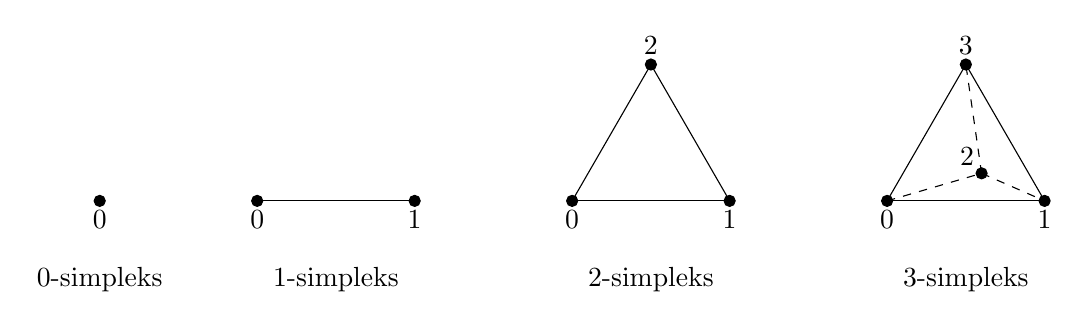
\begin{tikzpicture}
% ####################   0 - simplex    ####################
		\filldraw[black] (0, 0) circle (2pt) node[black, below]{$0$};
		\draw (0, -1) node {$0$-simpleks};
% ####################   1 - simplex    ####################
		\filldraw[black] (2, 0) circle (2pt) node[black, below]{$0$};		
		\filldraw[black] (4, 0) circle (2pt) node[black, below]{$1$};
		\draw (2, 0) -- (4, 0);
		\draw (3, -1) node {$1$-simpleks};
% ####################   2 - simplex    ####################
		\filldraw[black] (6, 0) circle (2pt) node[black, below]{$0$};		
		\filldraw[black] (8, 0) circle (2pt) node[black, below]{$1$};
		\filldraw[black] (7, 1.732) circle (2pt) node[black, above]{$2$};
		\draw (6, 0) -- (8, 0);
		\draw (6, 0) -- (7, 1.732);
		\draw (7, 1.732) -- (8, 0);
		\draw (7, -1) node {$2$-simpleks};
% ####################   3 - simplex    ####################
		\filldraw[black] (10, 0) circle (2pt) node[black, below]{$0$};		
		\filldraw[black] (12, 0) circle (2pt) node[black, below]{$1$};
		\filldraw[black] (11.2, 0.35) circle (2pt) node[black, above left = -0.4mm]{$2$};
		\filldraw[black] (11, 1.732) circle (2pt) node[black, above]{$3$};				
		\draw (10, 0) -- (12, 0);
		\draw (10, 0) -- (11, 1.732);
		\draw (11, 1.732) -- (12, 0);
		\draw[dashed] (10, 0) -- (11.2, 0.35);
		\draw[dashed] (11.2, 0.35) -- (11, 1.732);
		\draw[dashed] (11.2, 0.35) -- (12, 0);
		\draw (11, -1) node {$3$-simpleks};
	\end{tikzpicture}
	
\end{document}